\documentclass[letterpaper,11pt]{article}
\usepackage{graphicx}
\usepackage{listings}
\usepackage[super]{nth}
\usepackage[hyphens]{url}
\usepackage{hyperref}
\usepackage{amsmath}
\usepackage[makeroom]{cancel}
\usepackage[table]{xcolor}
\usepackage{comment}
\usepackage[space]{grffile}

\newcommand*{\srcPath}{../src}%
\lstset{
	basicstyle=\footnotesize,
	breaklines=true,
}

\begin{document}

\begin{titlepage}

\begin{center}

\Huge{Assignment 2}

\Large{CS 532:  Introduction to Web Science}

\Large{Spring 2018}

\Large{Hrishikesh Gadkari}

\Large Finished on \today

\end{center}

\end{titlepage}

\newpage


% =================================
% First question
% =================================
\section*{1}


\subsection*{Question}

\begin{verbatim}
1.  Write a Python program that extracts 1000 unique links from
Twitter.  You might want to take a look at:

http://adilmoujahid.com/posts/2014/07/twitter-analytics/

see also:

http://docs.tweepy.org/en/v3.5.0/index.html
https://github.com/bear/python-twitter
https://dev.twitter.com/rest/public

But there are many other similar resources available on the web.
Note that only Twitter API 1.1 is currently available; version 1
code will no longer work.

Also note that you need to verify that the final target URI (i.e.,
the one that responds with a 200) is unique.  You could have many
different shortened URIs for www.cnn.com (t.co, bit.ly, goo.gl,
etc.).  For example:

$ curl -IL --silent https://t.co/DpO767Md1v | egrep -i "(HTTP/1.1|^location:)"
HTTP/1.1 301 Moved Permanently
location: https://goo.gl/40yQo2
HTTP/1.1 301 Moved Permanently
Location: https://soundcloud.com/roanoketimes
/ep-95-talking-hokies-recruiting-one-week-before-signing-day
HTTP/1.1 200 OK
You might want to use the search feature to find URIs, or you can
pull them from the feed of someone famous (e.g., Tim O'Reilly).  If
you find something inappropriate for any reason you see fit, just
discard it and get some more links.  We just want 1000 links that
were shared via Twitter.
Hold on to this collection and upload it to github -- we'll use it
later throughout the semester.
\end{verbatim}
\subsection*{Answer}
To solve the above problem, I first went through the two resources \cite{twitterref} and \cite{twitterstreamref} as mentioned on the assignment page as well as from the discussion in the class, I got to know that in order to access the twitter API and fetch URIs I need to get keys and tokens by creating a developer account on twitter.
Also, the program needed to install and import tweepy library which allows the developer to stream tweets based on keywords. The following dependencies were used:
\begin{itemize}
  \item from tweepy.streaming import StreamListener
  \item from tweepy import OAuthHandler
  \item from tweepy import Stream
  \item import json
  \item import requests
  \item import urllib
  \item	import tldextract
  \item	from urllib.parse import urlparse, urljoin
  \item	import sys

\end{itemize}
For this assignment I reused the code which was developed for assignment 2 which made implementation much easier and quicker. The program shown in Listing \ref{lst:q1tweepy} was written in Python 3.5 for fetching 1000 unique links, omitting links from twitter domain. The following command was used to run and save the output in \textbf{1000ulinks.txt}.
\begin{lstlisting}[frame=single]
python tweet_crawl.py > 1000ulinks.txt
\end{lstlisting}

\lstinputlisting[frame=single,caption={Python script for twitter streaming},label=lst:q1tweepy,captionpos=b,numbers=left,showspaces=false,breakindent=0.5pt,showstringspaces=false,basicstyle=\footnotesize]{tweet_crawl.py}
For my keywords I chose the ones which were currently trending on twitter. It first starts by listening to the stream of data from twitters streaming API, from which data is received in JSON format. The data was parsed using entities and urls object of a tweet and also filtered them for lengths and maximum characters \cite{streamref}. These links one by one were sent to getLinksFromTweet for further filtration.
In the next step, HTTP head and get requests \cite{urllibref} were made for each of the links fetched from the previous step and checked if expandedUrl entity had any redirects or were shortened for status 200 as well as status 301. Next I used the tldextract \cite{tlderef} library for extracting the domain name as twitter since it had to be excluded. For checking the links to  be unique I maintained two lists where in List 1,  I stored all the URIs by formatting the query and parameters in links and List 2 where new links after comparing with List 1 , the links were again formed as original URIs. For this I used the urlparse and urljoin libraries \cite{parseref}.
\clearpage
% =================================
% Second question
% =================================
\section*{2}
\subsection*{Question}
\begin{verbatim}
2.  Download the TimeMaps for each of the target URIs.  We'll use the ODU 
Memento Aggregator, so for example:
URI-R = http://www.cs.odu.edu/
URI-T = http://memgator.cs.odu.edu/timemap/link/http://www.cs.odu.edu/
or:
URI-T = http://memgator.cs.odu.edu/timemap/json/http://www.cs.odu.edu/
(depending on which format you'd prefer to parse)
Create a histogram* of URIs vs. number of Mementos (as computed
from the TimeMaps).  For example, 100 URIs with 0 Mementos, 300
URIs with 1 Memento, 400 URIs with 2 Mementos, etc.  The x-axis
will have the number of mementos, and the y-axis will have the
frequency of occurence.
* = https://en.wikipedia.org/wiki/Histogram
What's a TimeMap?  
See: http://www.mementoweb.org/guide/quick-intro/
And the week 4 lecture. 
\end{verbatim}
\clearpage
\subsection*{Answer}
To solve the above problem,  \url{http://memgator.cs.odu.edu/} was used as mentioned in the question for getting the time maps for each of the 1000 URIs. I chose the JSON format to parse the data. The following dependencies were used:
\begin{itemize}
  \item import requests
  \item import json
  \item import os
  \item import csv
  
\end{itemize}  
First I checked the response code for first few URIs. From that I came to know about the links which had zero or no mementos, returned a response code of 404. So I made HTTP get and head requests to get the json data of timemaps and saved in .json file for URIs which returned 200 response using json.dump \cite{jsonref} function and in .txt file as No-Mementos for those which returned a 404 response.
Secondly to store the number of mementos and no of URIs in a csv file \cite{csvref} named \textbf{timemaps.csv}, I used a dictionary to arrange them with respect to Key as MementoCount and URICount as value.
The following program was written to implement the above problem in Python 3.5:
\lstinputlisting[frame=single,caption={Python Script for downloading Timemaps},label=lst:q2timemapPy,captionpos=b,numbers=left,showspaces=false,showstringspaces=false,basicstyle=\footnotesize]{timemap.py}
There were few errors while plotting the histogram, for which I had to write a small piece of code shown below, for converting the \textbf{timemaps.csv} file into a single column file named \textbf{counts.csv}.
\lstinputlisting[frame=single,caption={Conversion },label=lst:q2convPy,captionpos=b,numbers=left,showspaces=false,showstringspaces=false,basicstyle=\footnotesize]{singleColumn.py}
I then created a simple histogram , using R \cite{histref}  shown in Listing \ref{lst:q2timemapR}, of URIs vs. Number of Mementos as shown in Figure \ref{fig:q2histogram}. From the histogram observation we come to know that majority of URIs had zero or low counts of mementos.

\lstinputlisting[frame=single,caption={R script for creating Histogram},label=lst:q2timemapR,captionpos=b,numbers=left,showspaces=false,showstringspaces=false,basicstyle=\footnotesize]{thist.R}
\begin{figure}[h]
\centering
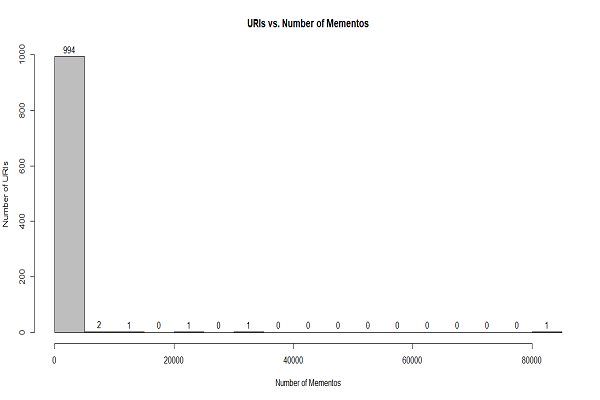
\includegraphics[scale=1.0]{memuri.png}
\caption{Histogram of Number of URIs vs. Number of Mementos}
\label{fig:q2histogram}
\end{figure}
\clearpage
% =================================
% Third question
% =================================
\section*{3}
\subsection*{Question}
\begin{verbatim}
3.  Estimate the age of each of the 1000 URIs using the "Carbon
Date" tool:
http://ws-dl.blogspot.com/2016/09/2016-09-20-carbon-dating-web-version-30.html
Note: you should use "docker" and install it locally.  You can do
it like this:
http://cd.cs.odu.edu/cd?url=http://www.cs.odu.edu/
But it will inevitably crash when everyone tries to use it at the
last minute.
For URIs that have > 0 Mementos and an estimated creation date,
create a graph with age (in days) on the x-axis and number of
mementos on the y-axis.
Not all URIs will have Mementos, and not all URIs will have an
estimated creation date.  Show how many fall into either categories.
For example,
total URIs:         1000
no mementos:     137  
no date estimate:  212
\end{verbatim}
\clearpage
\subsection*{Answer}
To solve the above problem, used the carbon dating tool \cite{carbondateref} provided in the question to retrieve the estimated creation dates and memgator to fetch the number of memtos for each of the URIs from the saved \textbf{1000ulinks.txt} file. I first checked first few links and came to know that links with zero mementos either no creation date or had a creation date whereas URIs that had no date estimates didn't contain any mementos. 
The following dependencies were used:
\begin{itemize}
  \item import requests
  \item import json
  \item from datetime import datetime
  \item import csv
  
\end{itemize}  

The program shown in Listing \ref{lst:q2carbonpy} was written in Python 3.5 and the output was saved in \textbf{dates.csv} while with column names as Age and MementoCount.

\lstinputlisting[frame=single,caption={Python script for finding the carbon date},label=lst:q2carbonpy,captionpos=b,numbers=left,showspaces=false,showstringspaces=false,basicstyle=\footnotesize]{carbon.py}
\clearpage
Also the program in Listing \ref{lst:q2carbonpy}, calculated the following values and saved in \textbf{calc.csv} file.
\begin{itemize}
  \item total URIs:	     1000
  \item no mementos:      533
  \item no date estimate: 82
\end{itemize}

The following R \cite{scatref} program was used to create the scatterplot  for Age in Days vs number of Mementos, shown in Figure \ref{fig:scatterplot}


\lstinputlisting[frame=single,caption={R Script to create scatterplot},label=lst:q2carbonDateR,captionpos=b,numbers=left,showspaces=false,showstringspaces=false,basicstyle=\footnotesize]{age.R}
\begin{figure}[h]
\centering
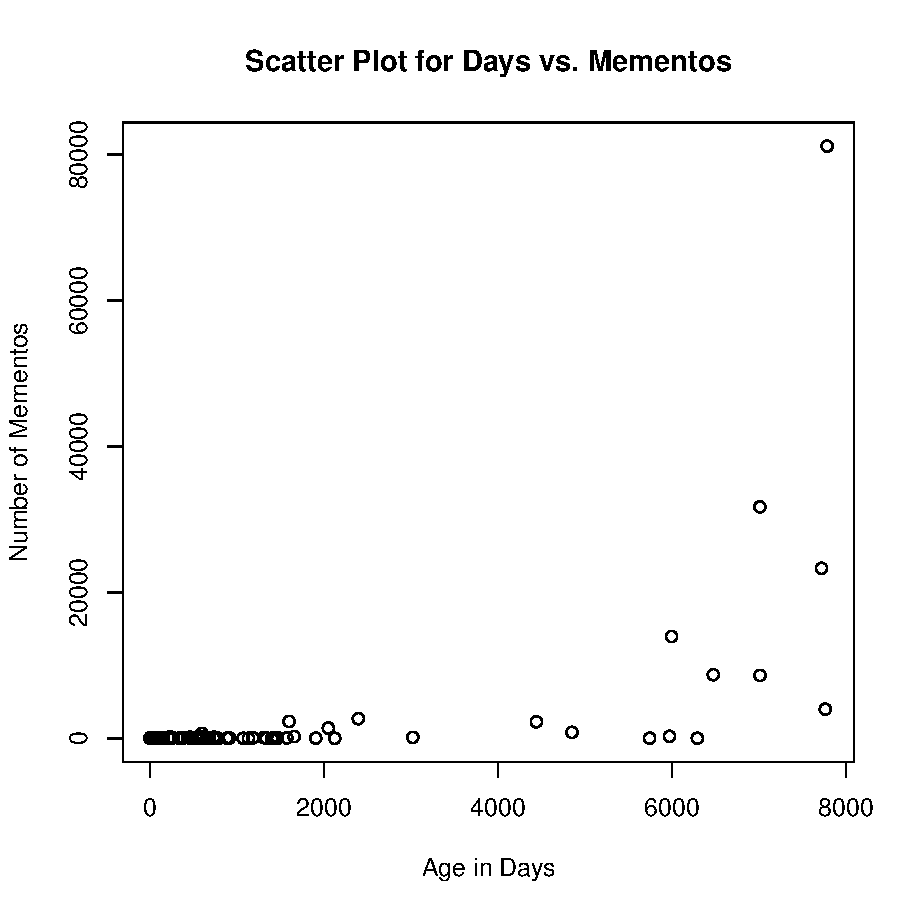
\includegraphics[scale=1.0]{ageuri.pdf}
\caption{Scatter plot of age in days and number of mementos}
\label{fig:scatterplot}
\end{figure}
\clearpage
% =================================
% Bibliography
% =================================
\begin{thebibliography}{9}
\bibitem{twitterref}
Python Programmng. ``Twitter API Streaming.''  N.p., 13 Feb. 2018.\url{https://pythonprogramming.net/twitter-api-streaming-tweets-python-tutorial/}
\bibitem{twitterstreamref} 
Moujahid, Adil. ``An Introduction to Text Mining Using Twitter Streaming API and Python.'' An Introduction to Text Mining Using Twitter Streaming API and Python // Adil Moujahid // Data Analytics and More. N.p., 21 July 2014. Web. 13 Feb. 2018. \url{http://adilmoujahid.com/posts/2014/07/twitter-analytics/}
\bibitem{streamref} 
Tweepy Documentation. ``Tweepy Documentation - tweepy 3.5.0 .''  N.p., 13 Feb. 2018. \url{http://docs.tweepy.org/en/v3.5.0/index.html}
\bibitem{tlderef} 
Python Software Foundation. ``tldextract 2.2.0 : Python Package Index .''  N.p., 13 Feb. 2018. \url{https://pypi.python.org/pypi/tldextract}
\bibitem{jsonref} 
Python Software Foundation. ``19.2. json - JSON encoder and decoder - Python 3.6.4 documentation .''  N.p., 13 Feb. 2018. \url{https://docs.python.org/3/library/json.html}
\bibitem{csvref} 
Python Software Foundation. ``14.1. csv - CSV File Reading and Writing - Python 3.6.4 documentation.''  N.p., 13 Feb. 2018. \url{https://docs.python.org/3/library/csv.html}
\bibitem{parseref} 
Urllib.parse Documentation. ``21.8. urllib.parse — Parse URLs into components — Python 3.6.4 documentation, Web. 13 Feb. 2018. \url{https://docs.python.org/3/library/urllib.parse.html}
\bibitem{urllibref} 
 Urllib.requests Documentation.``Developer Interface — Requests 2.18.4 documentation", Web. 13 Feb, 2018. \url{https://docs.python.org/3.0/library/urllib.request.html}
\bibitem{histref} 
 R Documentation.``function | R Documentation graphics", Web. 13 Feb, 2018. \url{https://www.rdocumentation.org/packages/graphics/versions/3.4.3/topics/hist}
\bibitem{scatref} 
 R Documentation.``function | R Documentation lessR", Web. 13 Feb, 2018. \url{https://www.rdocumentation.org/packages/lessR/versions/2.5/topics/ScatterPlot}
\bibitem{carbondateref}
Zetan, Li. ``2016-09-20: Carbon Dating the Web, Version 3.0.'' 2016-09-20: Carbon Dating the Web, Version 3.0. N.p., 20 Sept. 2016. Web. 08 Feb. 2017. \url{http://ws-dl.blogspot.com/2016/09/2016-09-20-carbon-dating-web-version-30.html}
\end{thebibliography}
\end{document}